\chapter{Explanation of the Mobile Application}

\section{The Building Blocks}



The following sections will explain integral parts of the server and client part of the mobile application. A gist of the architecture is shown
in figure \ref{fig:bb}. As it can be seen, the mobile app represents the user participating in the experiment. As the experiment goes on,
mobile sensor data and responses to the data requests which are collected are periodically sent to the Kinvey Data Store. 
The users can choose to login into the FairDataShare Portal from their computer or the mobile app. Once the user is authenticated, the user request
is sent from the FairDataShare server to the Kinvey Data Store. Kinvey in turn fetches the appropriate data and gives it to the FairDataShare Server. This in turn structures the data so it can be easily readable, and pushes it to the user to see on the portal. The concept is similar for the Stakeholders, except they can only access the portal through the computer and not the mobile app.

\begin{figure}[ht!]
\centering
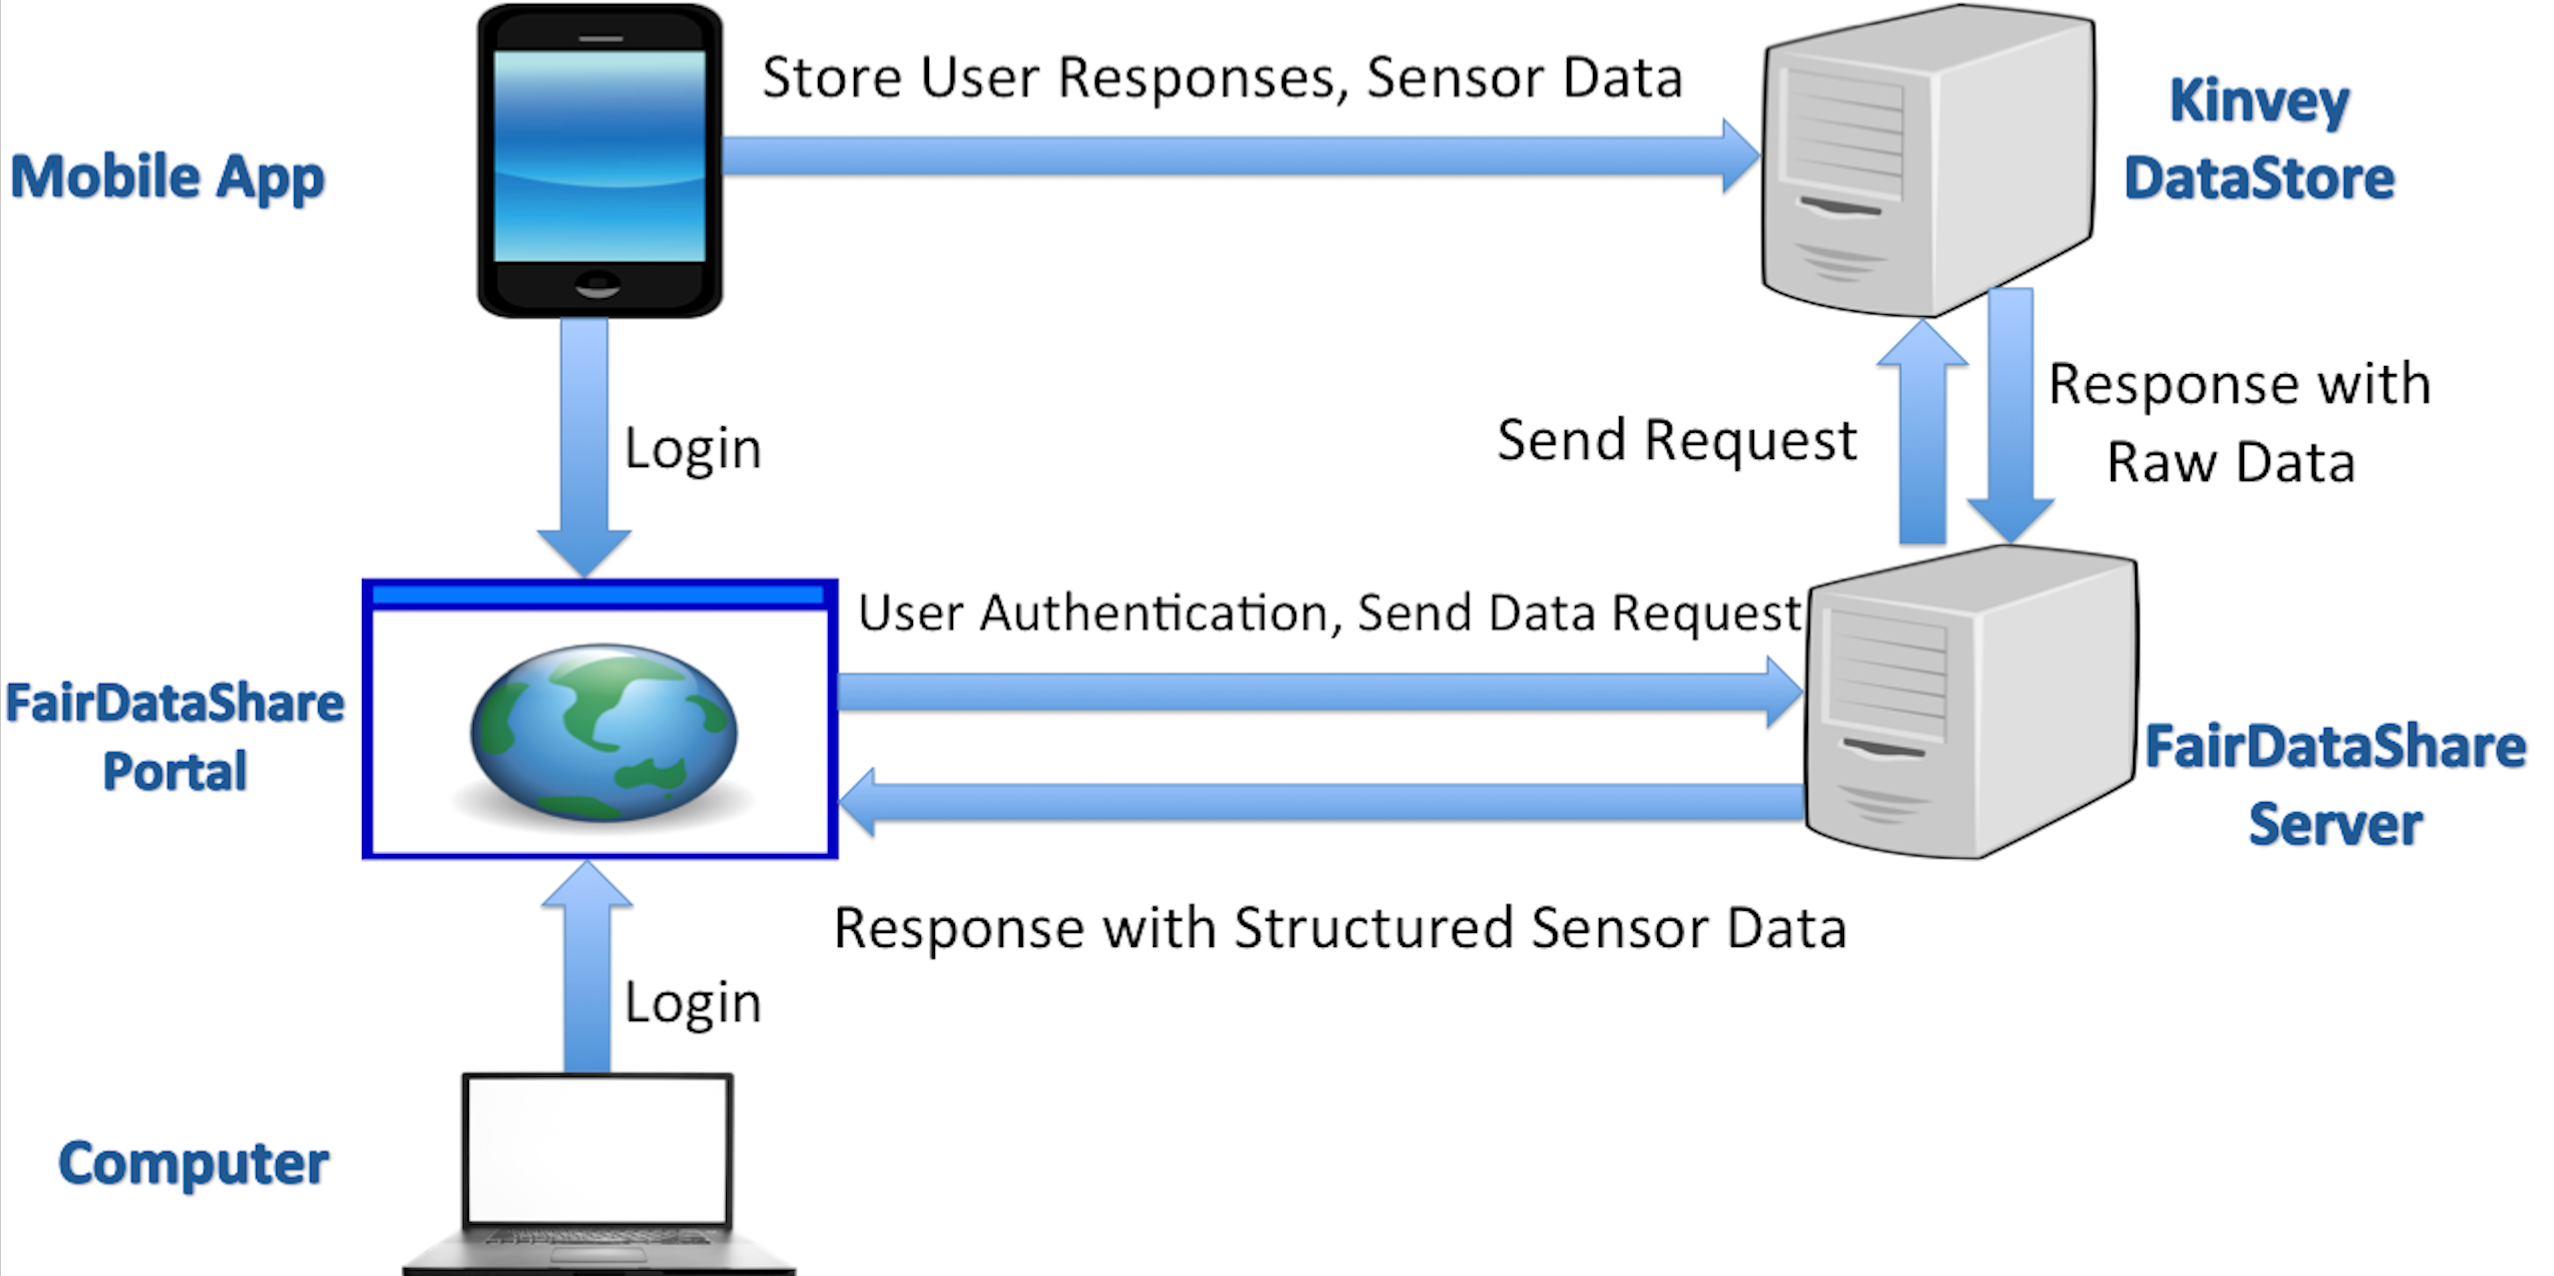
\includegraphics[width=\textwidth,keepaspectratio]{./images/blocks_app}
\caption{Conceptual Diagram of Mobile Application Architecture}
\label{fig:bb}
\end{figure}


\section{The Mobile Application}





\subsection{Local Storage}
the various db, schemas introduced, and why they are there


\begin{figure}[htp]
\subtop[Table Schema of QUESTIONSTORE\label{fig:db_quest}]{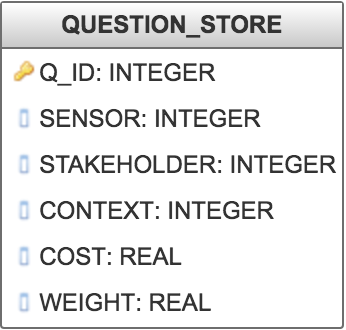
\includegraphics[width=0.4\linewidth]{./images/db_quest}}\hspace{1em}
\subtop[Table Schema of WHICHANSWERS\label{fig:db_which}]{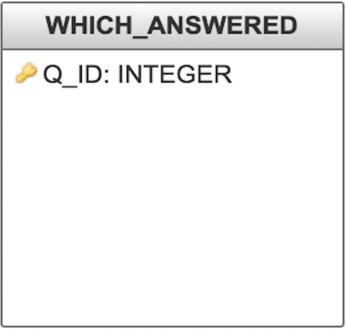
\includegraphics[width=0.4\linewidth]{./images/db_which_1}}
\caption{Table Schemas}
\label{fig:ts1}
\end{figure}


\begin{figure}[htp]
\subtop[Table Schema of STOREANSWERS\label{fig:db_ans}]{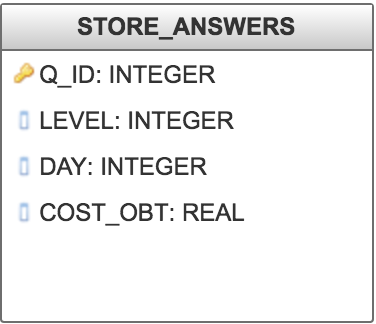
\includegraphics[width=0.4\linewidth]{./images/db_ans}} \hspace{1em}
\subtop[Table Schema of STOREANSWERS\label{fig:db_points}]{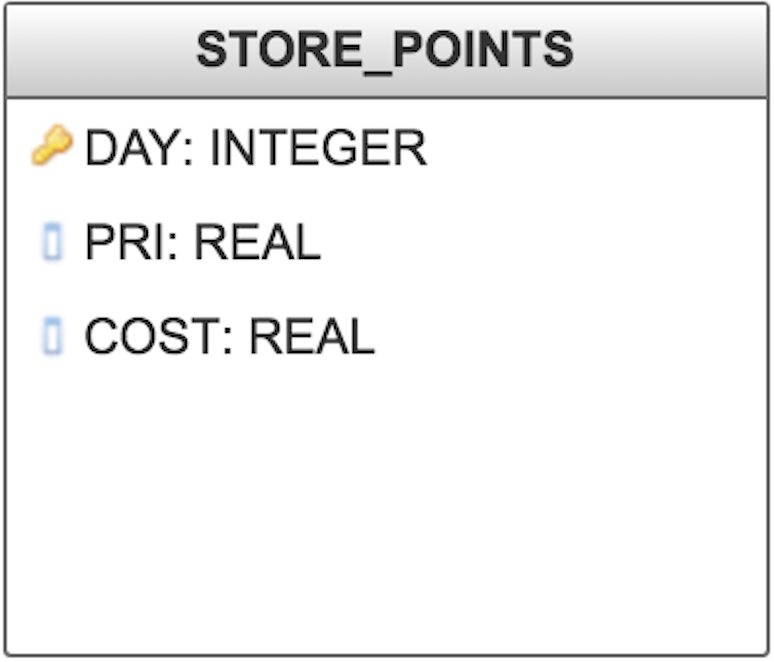
\includegraphics[width=0.4\linewidth]{./images/db_points}}
\caption{Table Schemas}
\label{fig:ts11}
\end{figure}




\begin{figure}[ht!]
\centering
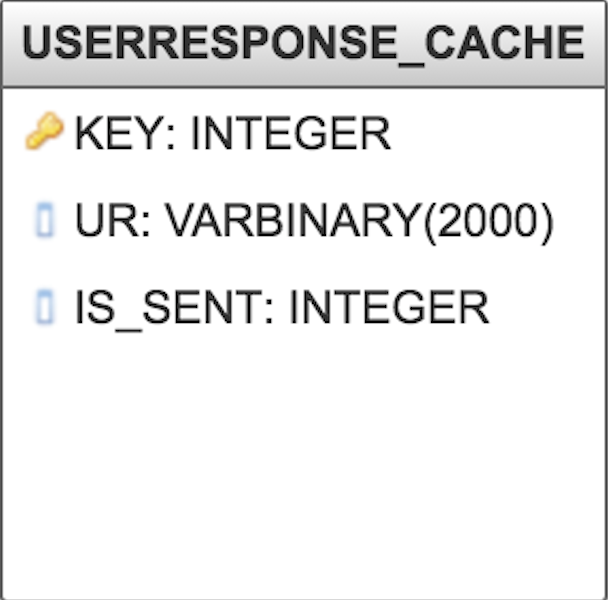
\includegraphics[width=0.4\linewidth]{./images/db_ur}
\caption{Table USERRESPONSECACHE Schema}
\label{fig:db_ur}
\end{figure}

\begin{figure}[htp]
\subtop[Table Schema of STOREACCELEROMETER\label{fig:db_acc}]{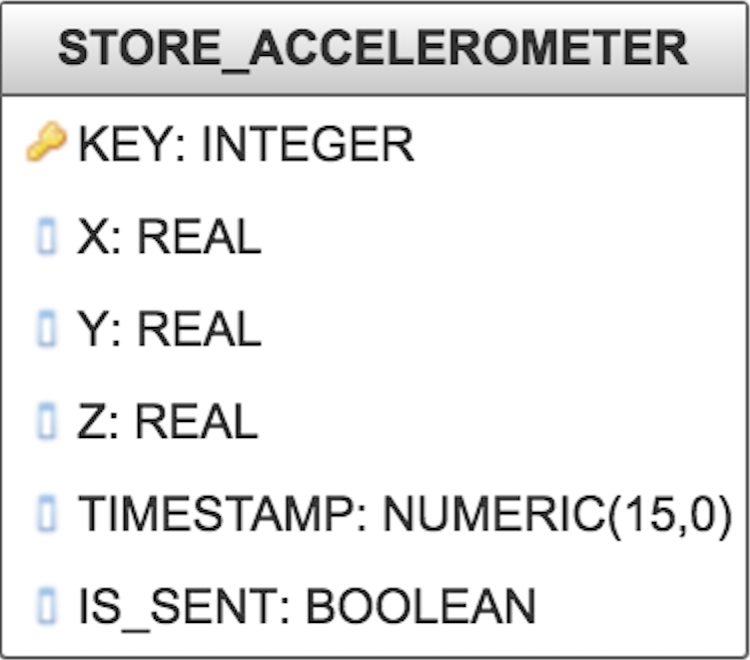
\includegraphics[width=0.4\linewidth]{./images/db_acc}}\hspace{1em}
\subtop[Table Schema of STORENOISE \label{fig:db_noise}]{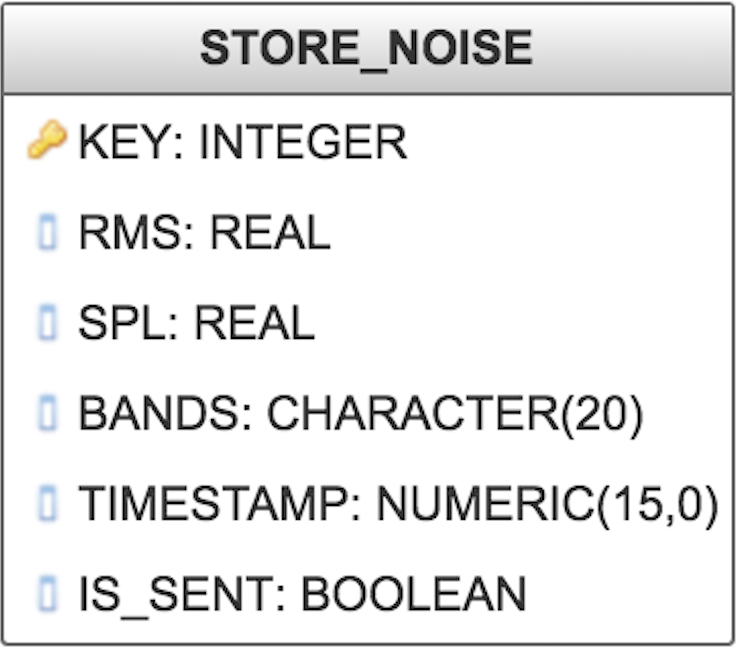
\includegraphics[width=0.4\linewidth]{./images/db_noise}}%
\caption{Table Schemas for Sensor Data}
\label{fig:ts2}
\end{figure}

\begin{figure}[htp]


\subtop[Table Schema of STORELOCATION\label{fig:db_loc}]{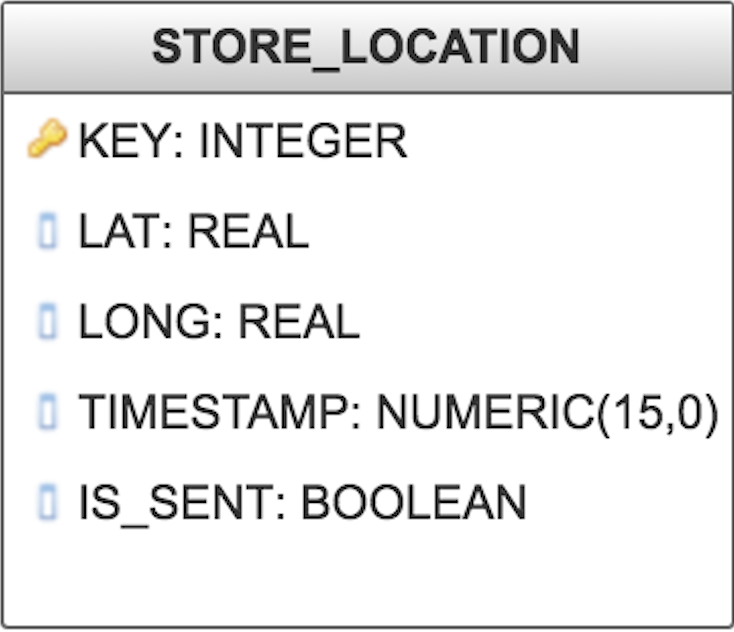
\includegraphics[width=0.4\linewidth]{./images/db_loc}}\hspace{1em}
\subtop[Table Schema of STORELIGHT \label{fig:db_light}]{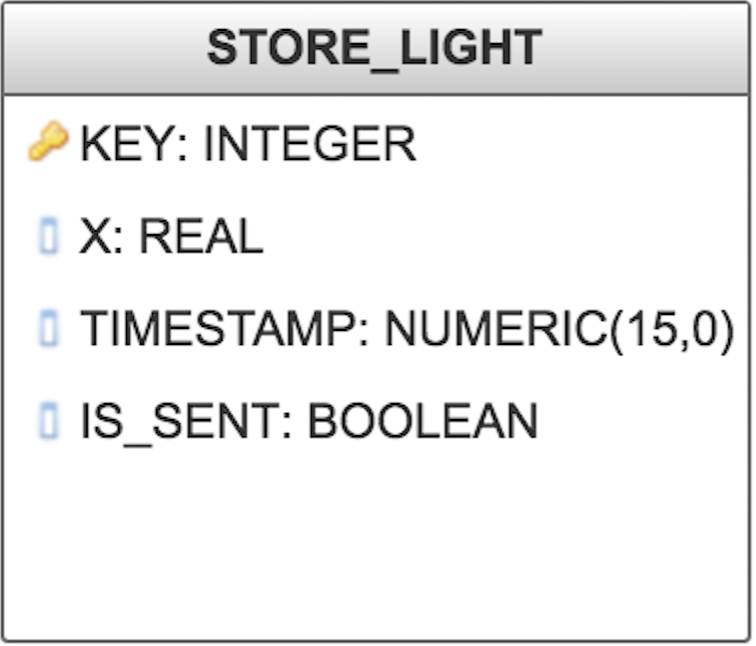
\includegraphics[width=0.4\linewidth]{./images/db_light}}%

\caption{Table Schemas for Sensor Data}
\label{fig:ts22}
\end{figure}

\subsection{Alarms and Notifications}

coping the alarms during rebooting, if alarms missing or not

\subsubsection{Going to the Next Data Sharing Day}
events thatt ake place when going to the next day


\subsection{Fetching Data Requests}




\subsection{Recording User Choices}

\subsection{Sensor Data Collection and Summarization}

\subsection{Server Synchronization}


\section{The Server}

\subsection{Kinvey Data Storage}

Kinvey is a mobile backend as a service which provides a platform for mobile phones to link applications at a backend cloud storage. This backend has been used to store data and for some business logic implementations.
\subsubsection{Security}

\subsubsection{Table Store}

\begin{figure}[ht!]
\centering
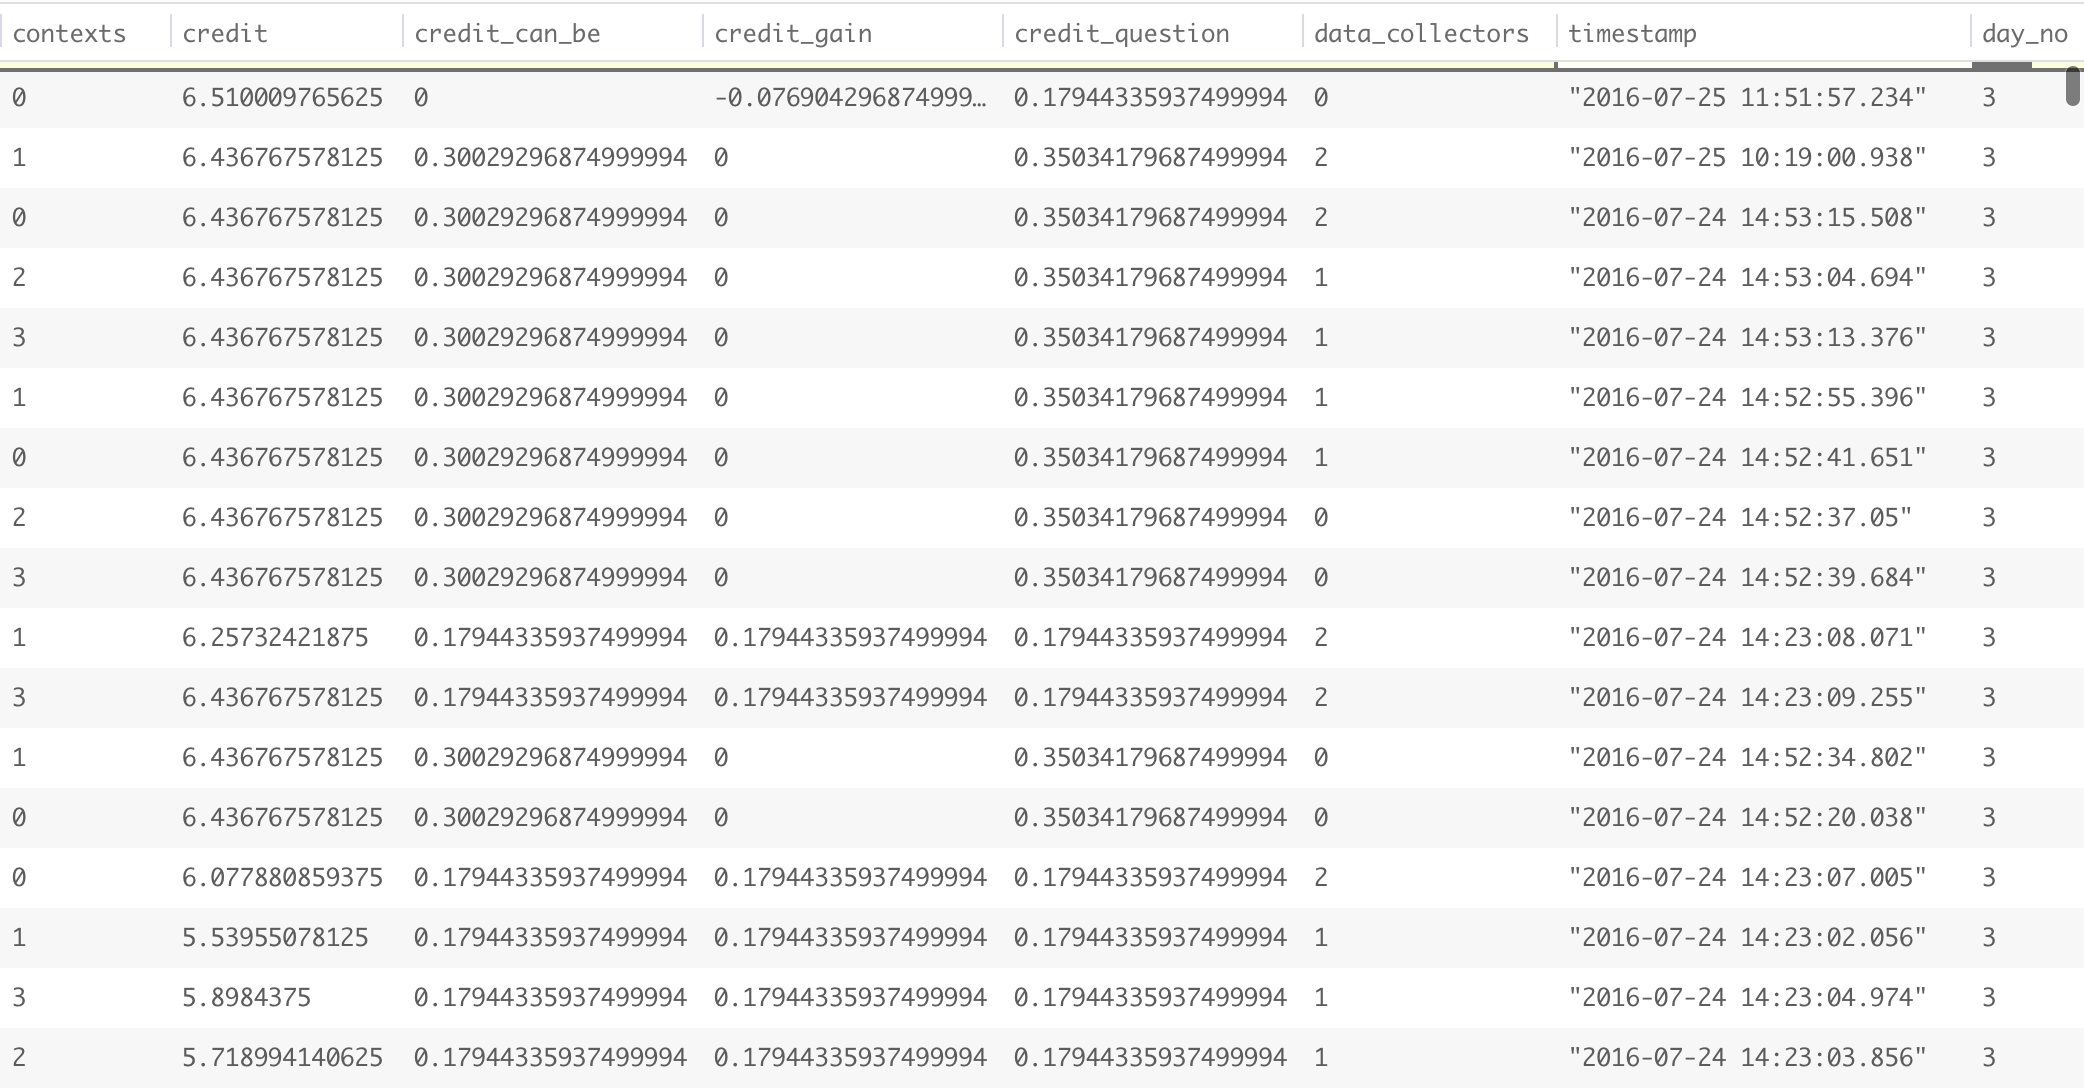
\includegraphics[width=\textwidth,keepaspectratio, height=0.6\textwidth]{./images/collection_ur_1}
\caption{Screenshot of Collection UserResponse Part 1}
\label{fig:col_ur_1}
\end{figure}

\begin{figure}[ht!]
\centering
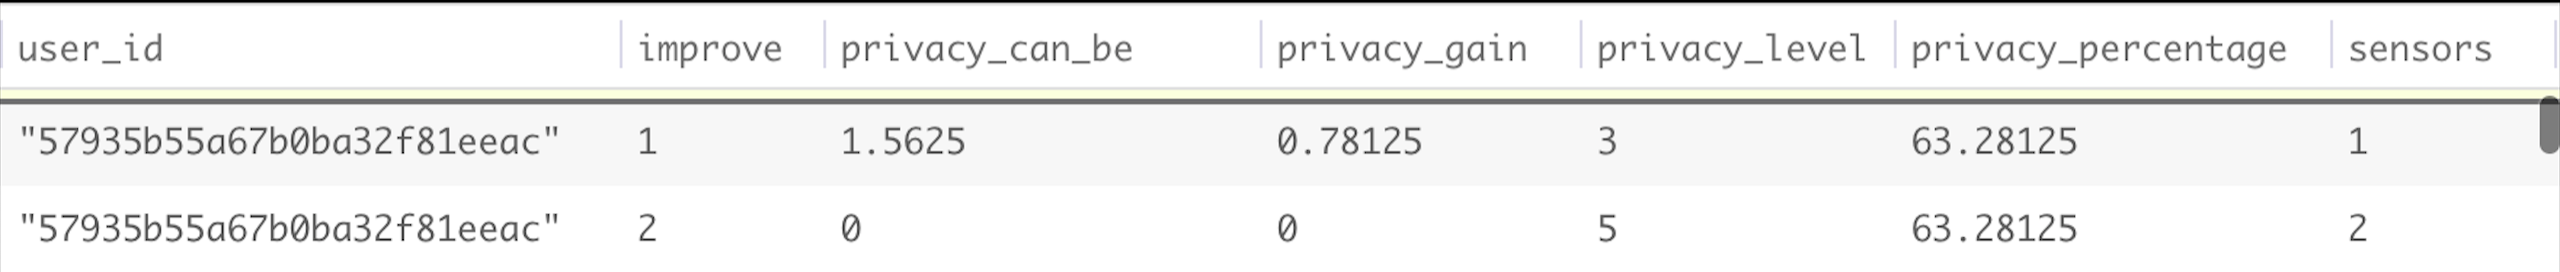
\includegraphics[width=\textwidth,keepaspectratio,height=0.6\textwidth]{./images/collection_ur_2}
\caption{Screenshot of Collection UserResponse Part 2}
\label{fig:col_ur_2}
\end{figure}

\begin{figure}[ht!]
\centering
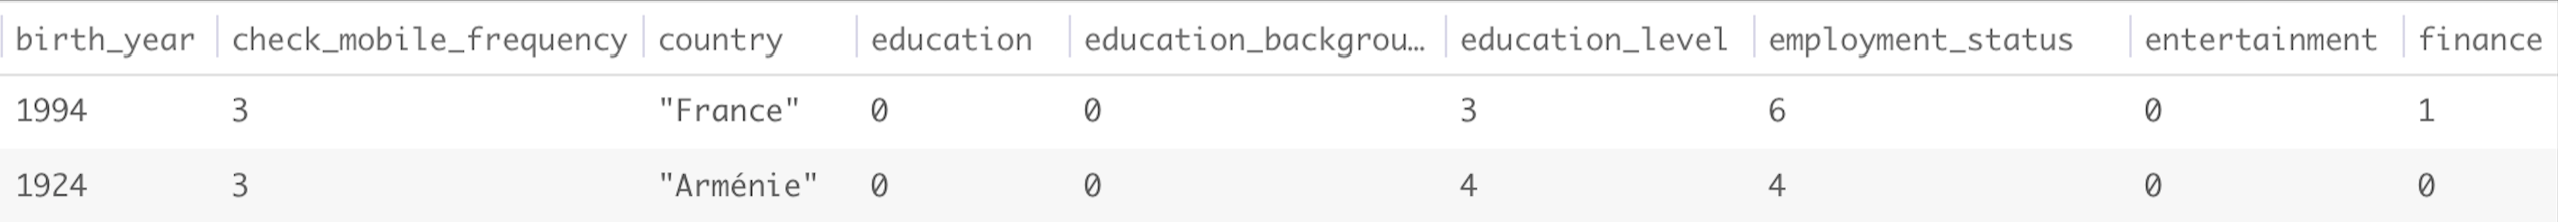
\includegraphics[width=\textwidth,keepaspectratio,height=0.6\textwidth]{./images/collection_ui_1}
\caption{Screenshot of Collection UserInformation Part 1}
\label{fig:col_ui_1}
\end{figure}

\begin{figure}[ht!]
\centering
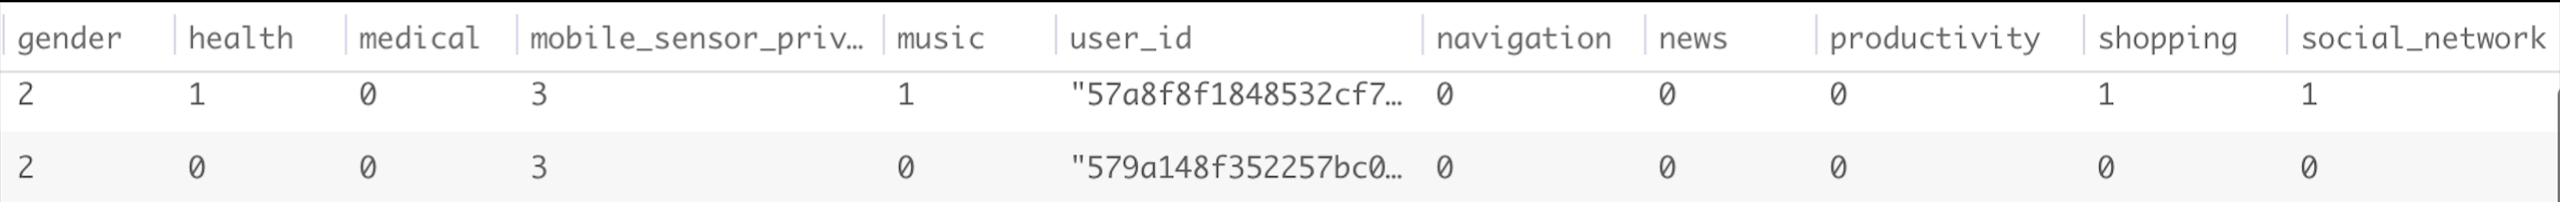
\includegraphics[width=\textwidth,keepaspectratio,height=0.6\textwidth]{./images/collection_ui_2}
\caption{Screenshot of Collection UserInformation Part 2}
\label{fig:col_ui_2}
\end{figure}

\begin{figure}[ht!]
\centering
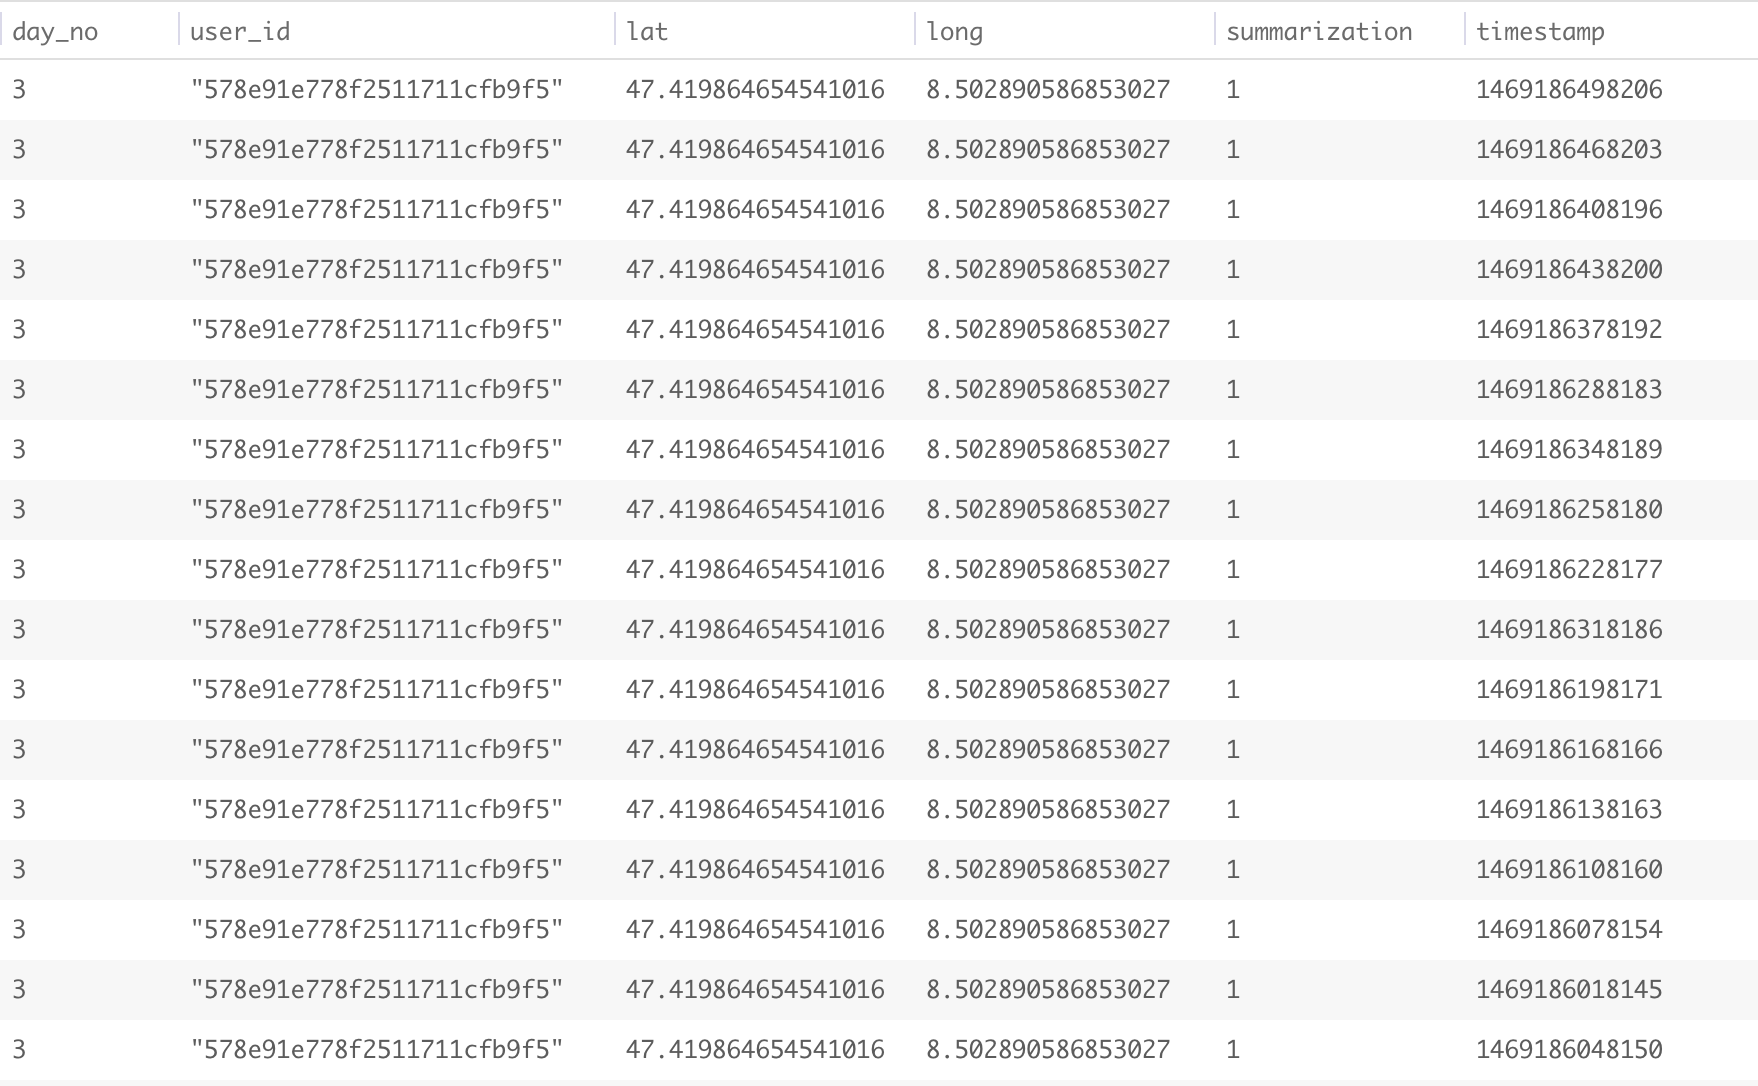
\includegraphics[width=\textwidth,keepaspectratio,height=0.6\textwidth]{./images/collection_loc}
\caption{Screenshot of Collection Location}
\label{fig:col_loc}
\end{figure}

\begin{figure}[ht!]
\centering
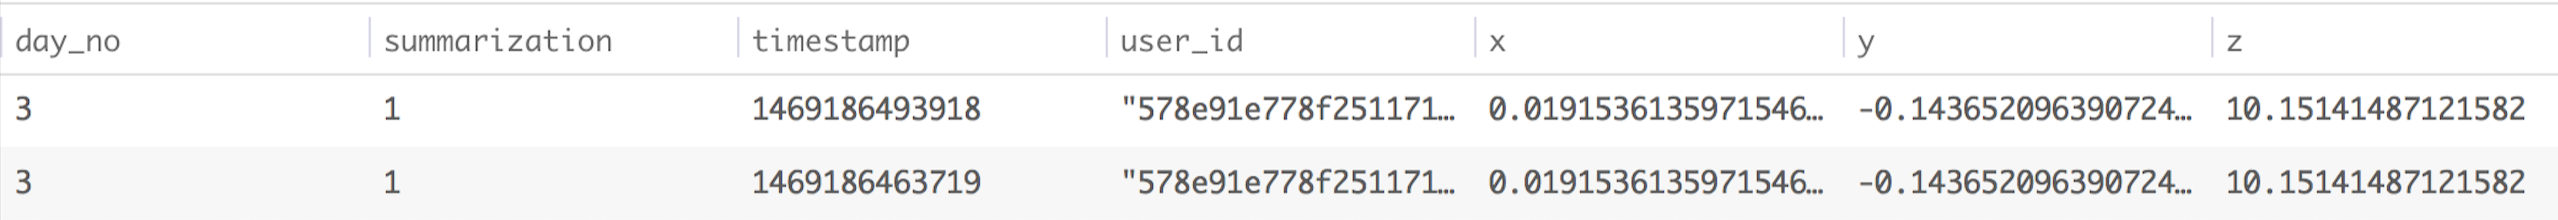
\includegraphics[width=\textwidth,keepaspectratio,height=0.6\textwidth]{./images/collection_acc}
\caption{Screenshot of Collection Accelerometer}
\label{fig:col_acc}
\end{figure}

\begin{figure}[ht!]
\centering
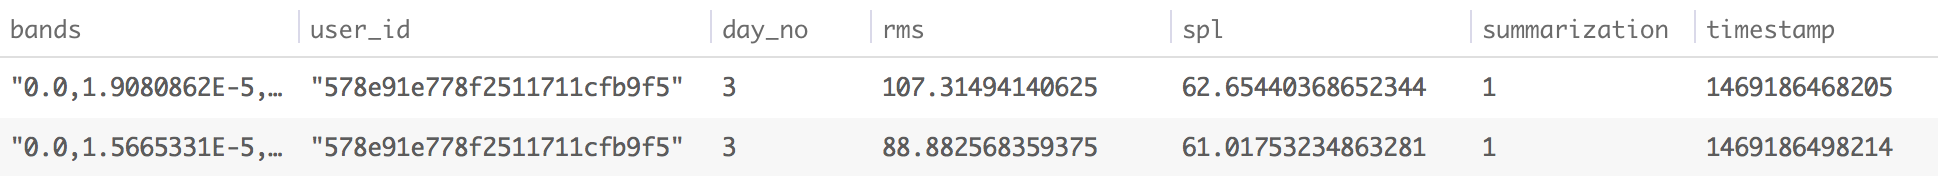
\includegraphics[width=\textwidth,keepaspectratio,height=0.6\textwidth]{./images/collection_noise}
\caption{Screenshot of Collection Noise}
\label{fig:col_noise}
\end{figure}

\begin{figure}[ht!]
\centering
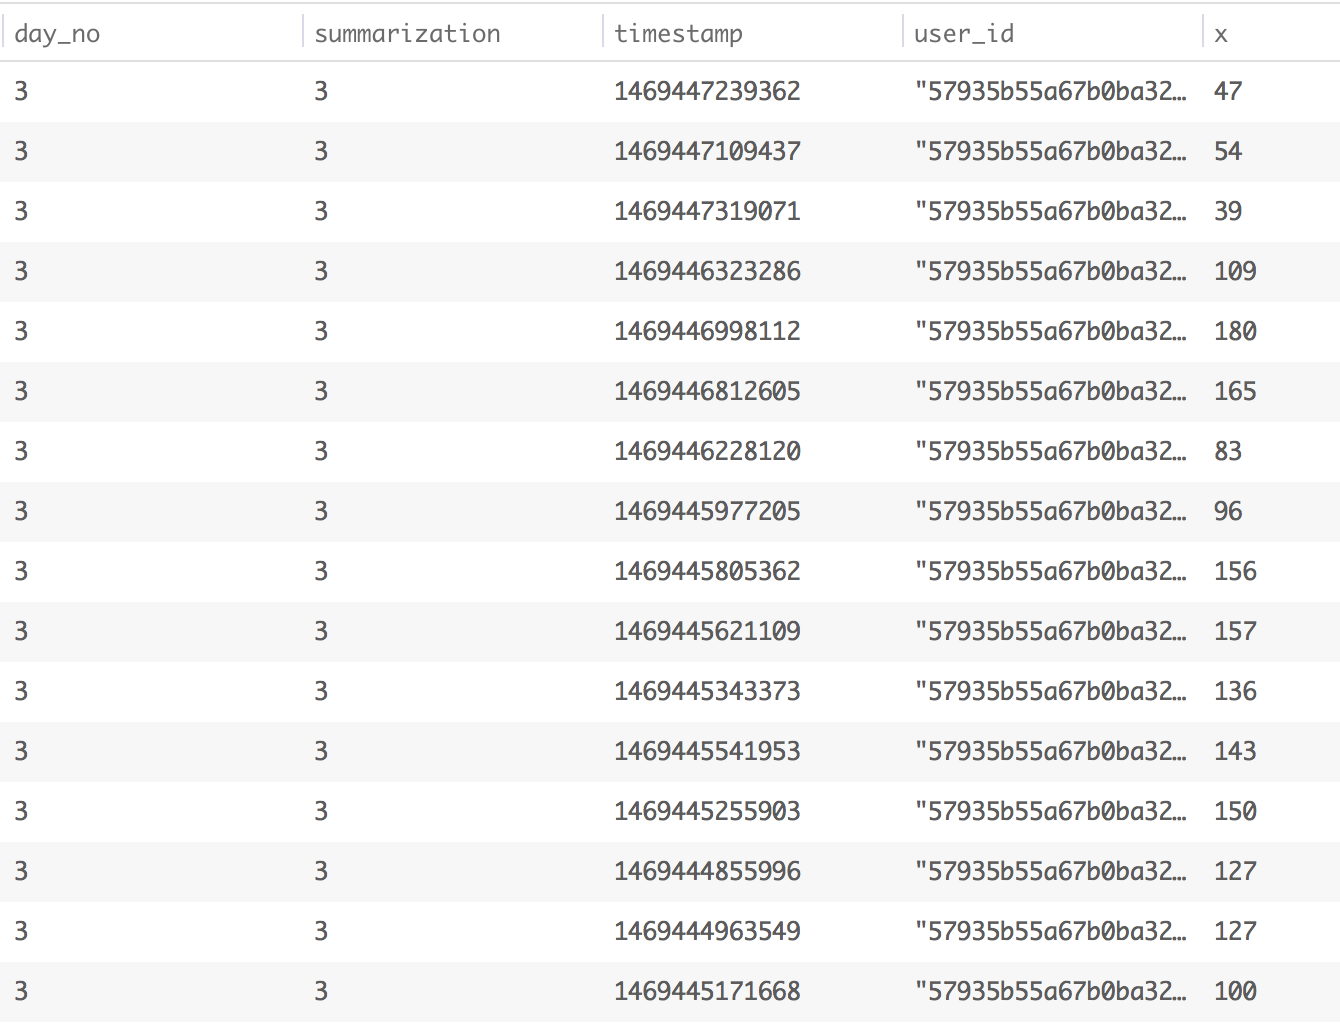
\includegraphics[width=\textwidth,keepaspectratio,height=0.6\textwidth]{./images/collection_light}
\caption{Screenshot of Collection Light}
\label{fig:col_light}
\end{figure}

\begin{figure}[ht!]
\centering
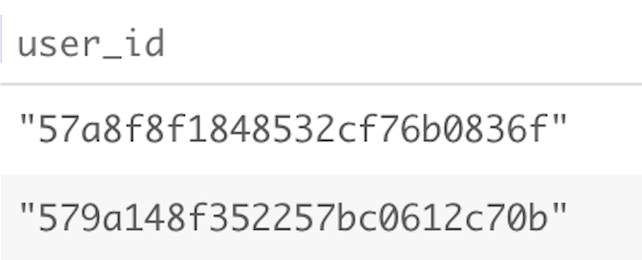
\includegraphics[width=\textwidth,keepaspectratio,height=0.6\textwidth]{./images/collection_users}
\caption{Screenshot of Collection Users}
\label{fig:col_users}
\end{figure}

\begin{figure}[ht!]
\centering
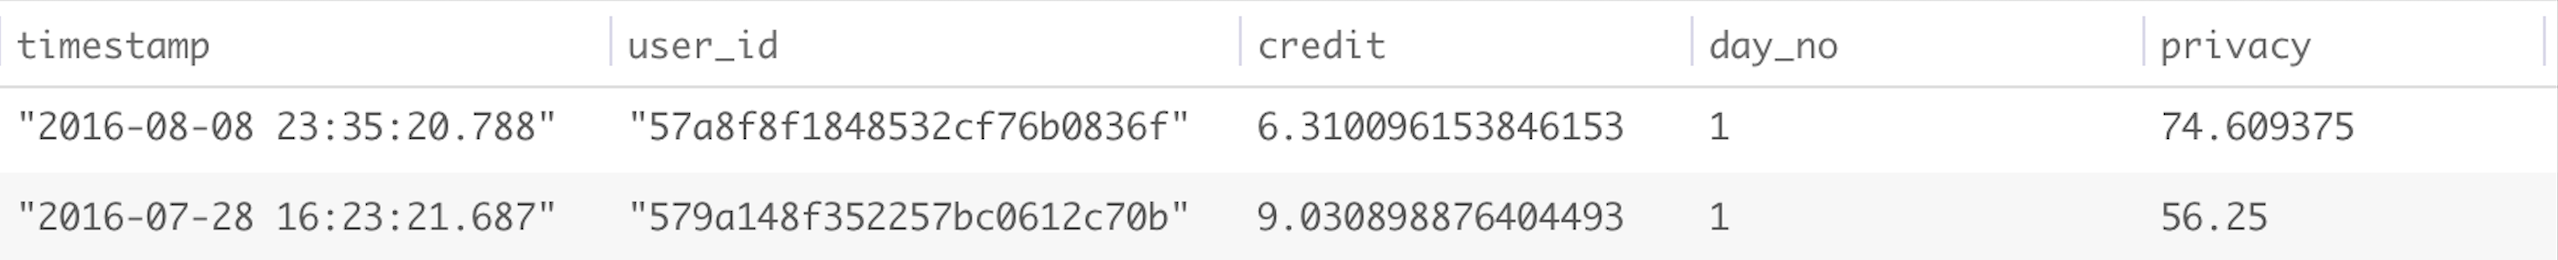
\includegraphics[width=\textwidth,keepaspectratio,height=0.6\textwidth]{./images/collection_score}
\caption{Screenshot of Collection Score}
\label{fig:col_score}
\end{figure}

\begin{figure}[ht!]
\centering
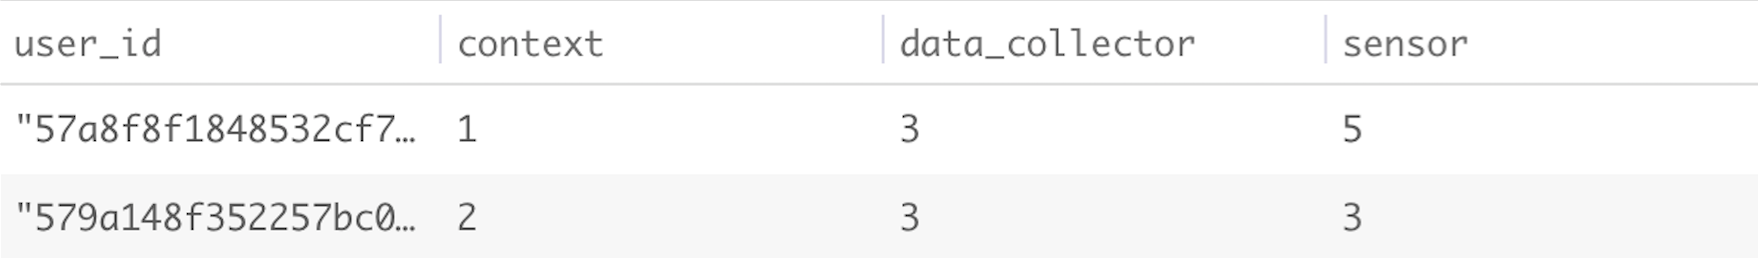
\includegraphics[width=\textwidth,keepaspectratio,height=0.6\textwidth]{./images/collection_feature_cat}
\caption{Screenshot of Collection Features}
\label{fig:col_f}
\end{figure}

\begin{figure}[ht!]
\centering
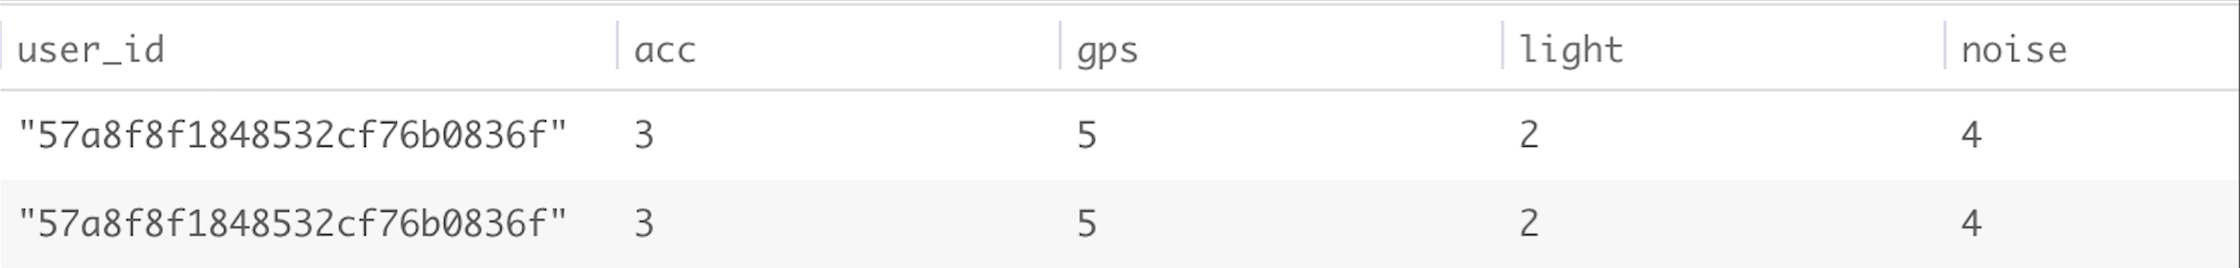
\includegraphics[width=\textwidth,keepaspectratio,height=0.6\textwidth]{./images/collection_sensors_cat}
\caption{Screenshot of Collection Sensors}
\label{fig:col_s}
\end{figure}

\begin{figure}[ht!]
\centering
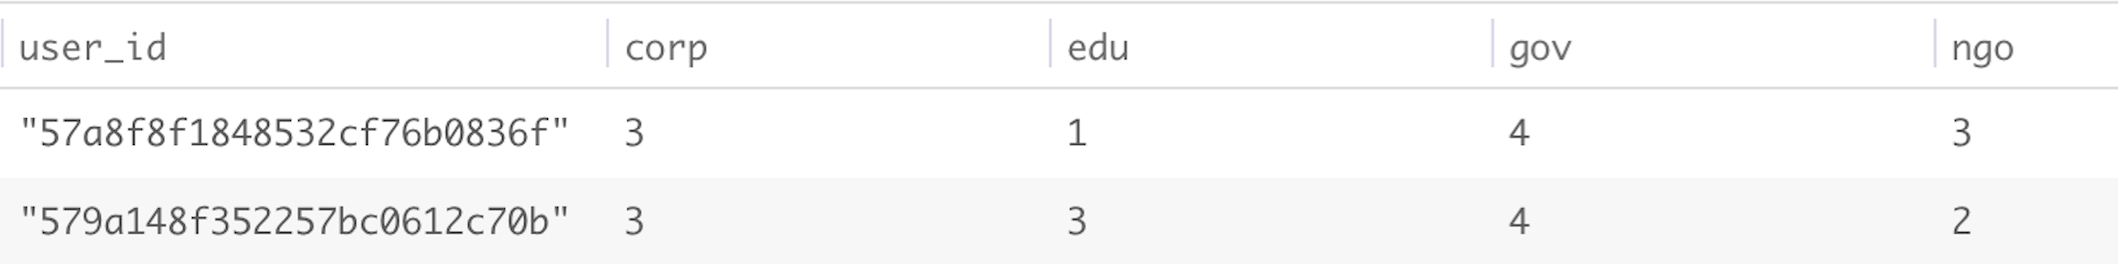
\includegraphics[width=\textwidth,keepaspectratio,height=0.6\textwidth]{./images/collection_dc_cat}
\caption{Screenshot of Collection Stakeholders}
\label{fig:col_ss}
\end{figure}

\begin{figure}[ht!]
\centering
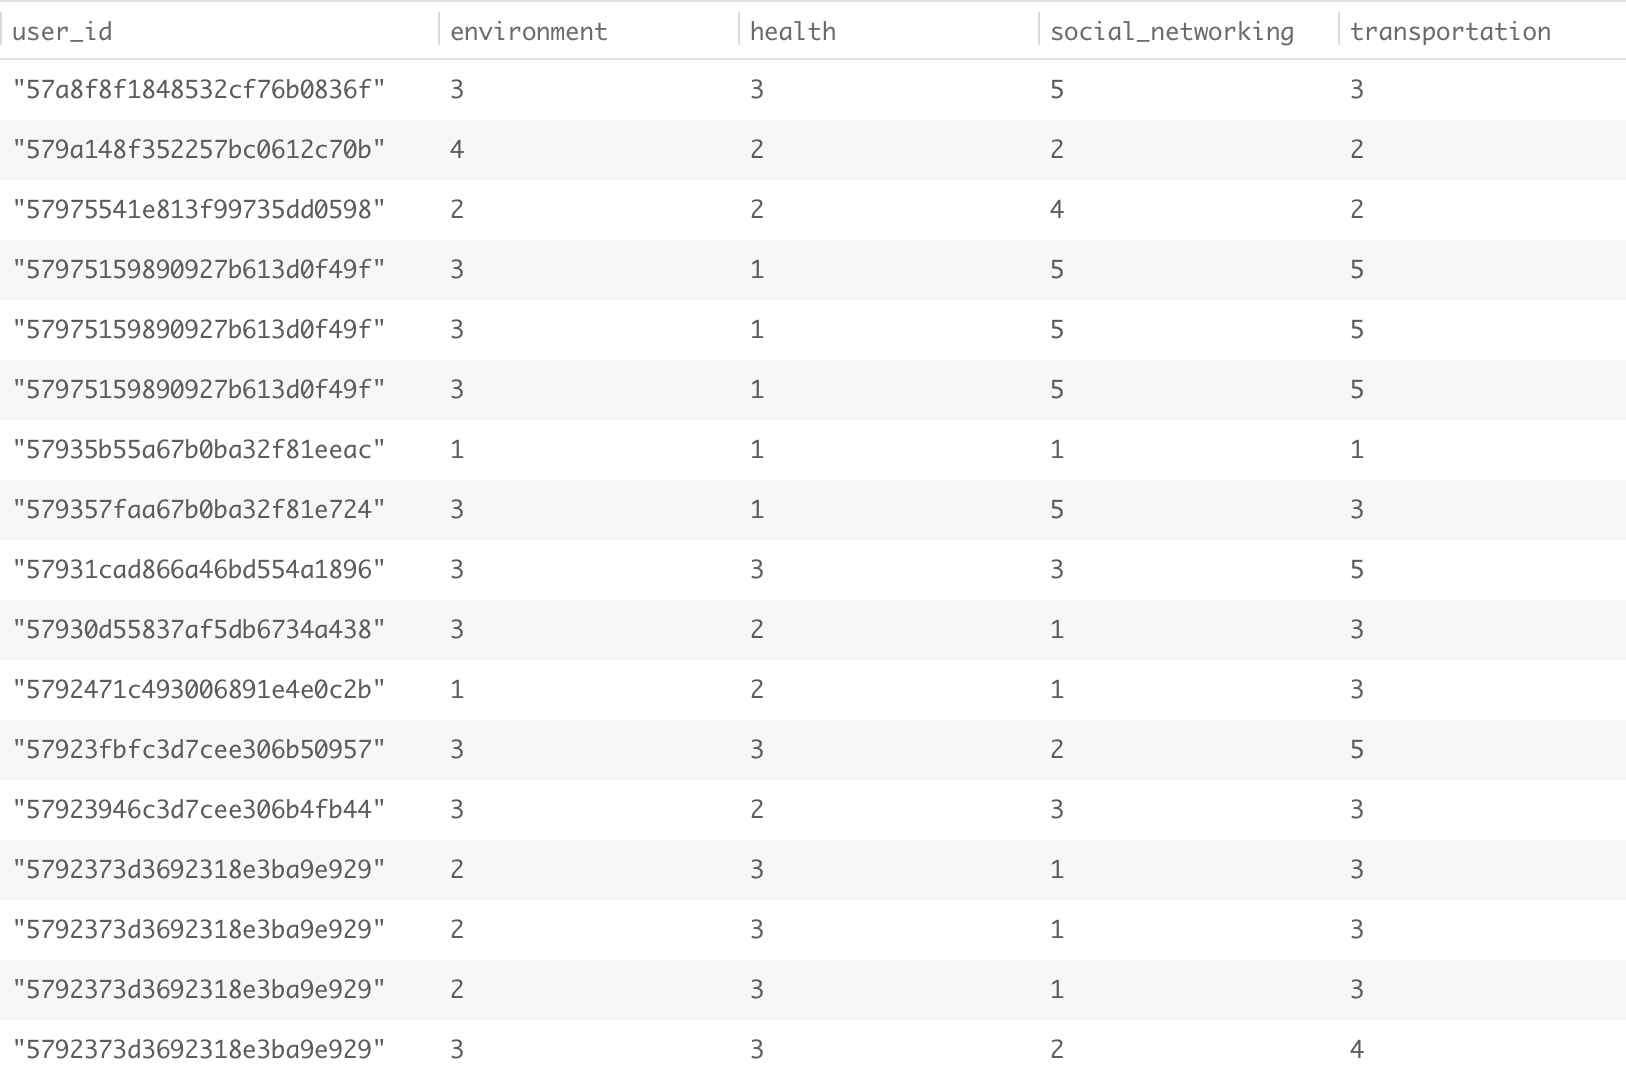
\includegraphics[width=\textwidth,keepaspectratio,height=0.6\textwidth]{./images/collection_context_cat}
\caption{Screenshot of Collection Contexts}
\label{fig:col_c}
\end{figure}

All the data collected form the user's phones is stored in Kinvey Data Store's collections. Data is segregated in to the appropriate collections. Data is stored in the collections is done so in the following form :

\begin{enumerate}
    \item Data collected in the form of radio buttons on the phone are stored as integers.
    \item Data collected as check-box entries on the phone each have a column in the collection with entries zero or one.
    \item Data collected as drop down lists on the phone are stored either by integer position in the list or by the entry name in the list itself.
\end{enumerate}

This way of storing data applies to all the collections explained below. Each record of every collection is with a unique user identifier and with the timestamp whenever necessary. This is done to identify data that belongs to the same user accross different collections. The timestamp
is collected in order to examine temporal relationships.
The first collection is the GetUserInformation collection and is used to store all the basic non intrusive user information 
collected in the entry phase. The collection is shown in figure \ref{}. Next, is the UserResponse collection which is used to store all
the responses of the users to data requests in the entry phase and the core phase. The collection is shown in figure \ref{}. Collection AccelerometerStore, LightStore, NoiseStore and LocationStore are used to store the mobile sensor data collected from the user at the end of a bidding day after local summarization on the mobile phone. Theses collections are shown in figures \ref{} \ref{} \ref{} \ref{}. The StorePoints collection is used to store the privacy and credit metrics obtained at the end of each bidding day  for each user and is shown in figure \ref{}.

\subsubsection{Bussiness Logic} \ref{bl}
Most of the bussiness logic used in the FairDataShare portal is present on Kinvey. Two things are done here:
\begin{enumerate}
    \item Finding privacy for a user
    \item Summarization
\end{enumerate}
Data collected from the user consists of mobile sensor data with the least amount of summarization. This prevents for repeatedly
collecting data from users and saves space and mobile data. Therefore, this mobile sensor data needs to be further summarized before being given to the stakeholder. To do this, we first have to find the most recent privacy setting from the UserResponseCollection. This is done due to the fact users can answer a data request more than once, hence we need to fish out the latest response for a particular sensor. Once this is done, using the recorded privacy level, we feed this input into another script that performs the summarization which has been explained in chapter \ref{model}.

\subsection{FairDataShare Web Portal}
The FairDataShare portal makes use of a server other Kinvey to safely store the usernames, passwords of users and the stakeholders. The database
technology used is MongoDB. The username and passwords are both stored in a collection. The language used to interact with Kinvey is Express.js, which is based on Node.js. Most of the data portal business logic is on Kinvey described in section \ref{bl}. The webpage was constructed using Html and css. Screenshots of the portal are provided in chapter \ref{exp}.









